\section{Pigeonhole Sort}

\subsection{Introduction}

\textbf{History:}
Peter Gustav Lejeune Dirichlet, who formally stated the idea in 1834.

\begin{figure}[H]
\centering
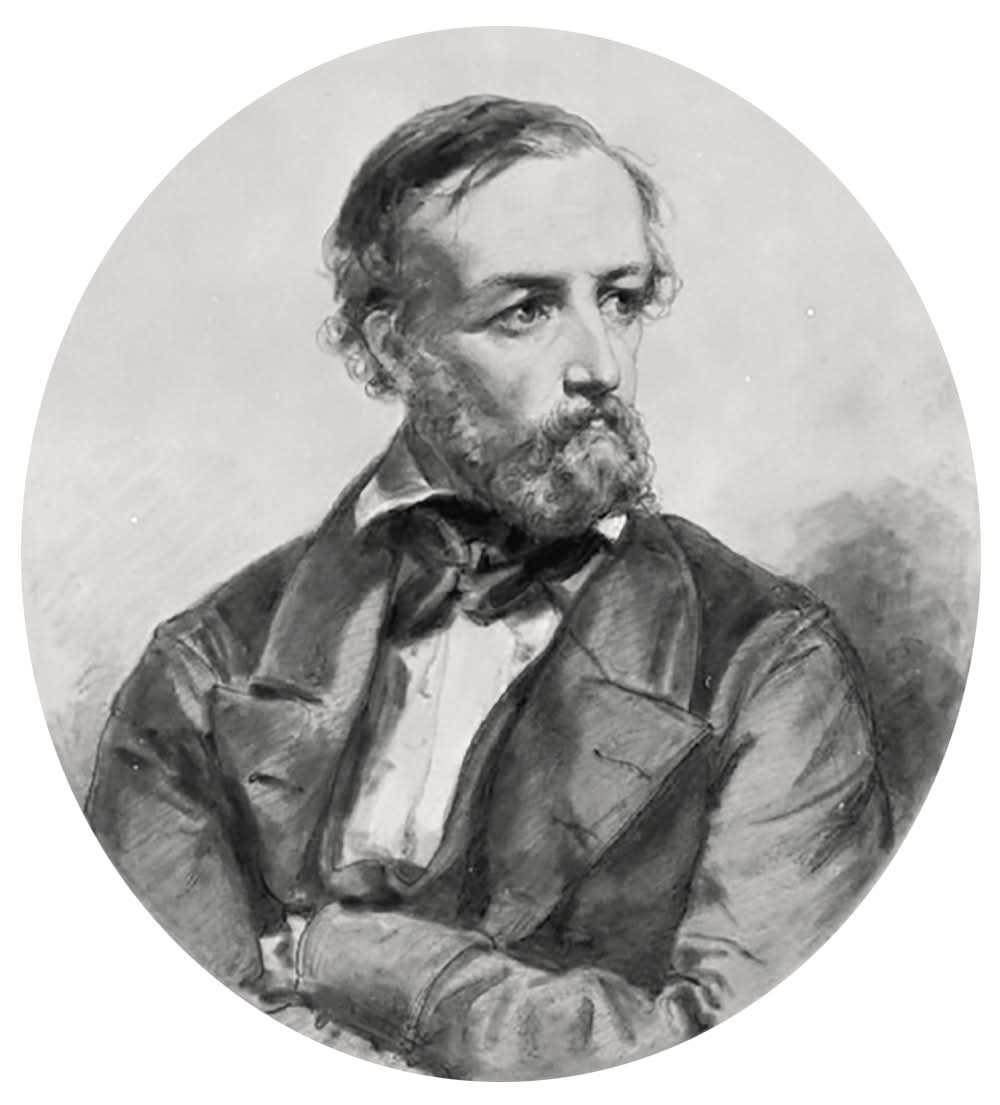
\includegraphics[scale=0.15]{img/pglDirichlet.jpg}
\caption{Peter Gustav Lejeune Dirichlet (1805-1859)}
\label{fig:pgl_dirichlet}
\end{figure}

\textbf{Definition:}
\begin{itemize}
    \item Pigeonhole sorting is a sorting algorithm that is suitable for sorting lists of elements where the number of elements and the number of possible key values are approximately the same.
    \item It requires $O(n + \text{Range})$ time where $n$ is the number of elements in the input array and ‘Range’ is the number of possible values in the array.
\end{itemize}

\subsection{Algorithm and Implementation}

Pigeonhole sort is similar to counting sort, but differs in that it “moves items twice: once to the bucket array and again to the final destination.”

\begin{enumerate}
    \item \textbf{Determine the range:} Find the minimum and maximum values in the array. Let the minimum and maximum values be ‘min’ and ‘max’ respectively. Also, find the range as ‘max-min+1’.
    \item \textbf{Initialize an array:} Set up an array of initially empty “pigeonholes” the same size as the range.
    \item \textbf{Distribution step:} Visit each element of the array and then put each element in its pigeonhole. An element $arr[i]$ is put in the hole at index $arr[i] - \text{min}$.
    \item \textbf{Output reconstruction phase:} Start the loop all over the pigeonhole array in order and put the elements from non-empty holes back into the original array.
\end{enumerate}

\begin{algorithm}
    \caption{Pigeonhole Sort}
    \begin{algorithmic}[1]
        \State \textbf{Input:} Array $A$ of size $n$
        \State \textbf{Output:} Sorted array $A$
        \Function{PigeonholeSort}{$A$, $n$}
        \State $min \gets \min(A)$
        \State $max \gets \max(A)$
        \State $range \gets max - min + 1$
        \State $P \gets \text{array of size } range \text{ initialized to 0}$
        \For{each element $x$ in $A$}
            \State $P[x - min] \gets P[x - min] + 1$
        \EndFor
        \State $index \gets 0$
        \For{$i \gets 0$ to $range - 1$}
            \While{$P[i] > 0$}
                \State $A[index] \gets i + min$
                \State $index \gets index + 1$
                \State $P[i] \gets P[i] - 1$
            \EndWhile
        \EndFor
        \EndFunction
    \end{algorithmic}
\end{algorithm}

Below is the implementation in C++:

\lstinputlisting[language=C++, caption=Pigeonhole Sort in C++, style=mystyle]{code/pigeonSort.cpp}

\subsection{Evaluation}

\subsubsection{Building the Pigeonhole Array}
\textbf{Operation:} Create and set up pigeonholes (buckets) for sorting the input array. \\
\textbf{Complexity:} \(O(n + \text{range})\) \\
\textbf{Explanation:} Each element in the input array is placed into its respective pigeonhole. The range refers to the difference between the maximum and minimum values.

\subsubsection{Filling the Pigeonhole Array}
\textbf{Operation:} Distribute elements from the input array into the pigeonholes. \\
\textbf{Complexity:} \(O(n)\) \\
\textbf{Explanation:} Traverse through the input array and assign each element to the appropriate pigeonhole.

\subsubsection{Reconstructing the Sorted Array}
\textbf{Operation:} Rebuild the sorted array by traversing through the pigeonholes in order. \\
\textbf{Complexity:} \(O(n + \text{range})\) \\
\textbf{Explanation:} Iterate over the pigeonholes and transfer elements back to the input array, ensuring the order is correct.

\subsubsection{Space Complexity Evaluation}
\textbf{Space Used:} \(O(\text{range})\) \\
\textbf{Explanation:} Additional memory is required to store the pigeonhole array, with its size being determined by the range of values in the input array (maximum value - minimum value + 1).

\subsection{Application}

Pigeonhole sort is a non-comparison-based sorting algorithm that works well for sorting integers or objects with small, discrete key ranges. It counts the occurrences of each element and uses this information to place elements in their correct sorted position.
\begin{enumerate}
    \item \textbf{Sorting Small Range Integers:} Pigeonhole sort is highly efficient for sorting integers or keys within a small, known range. \textit{Example:} Sorting exam scores (e.g., 0 to 100) or ages of individuals.
    \item \textbf{Histogram Generation:} Pigeonhole sort can be used to generate histograms or frequency distributions of data. \textit{Example:} Analyzing the frequency of words in a text or the distribution of pixel intensities in an image.
    \item \textbf{Data Compression:} Pigeonhole sort is used in data compression algorithms to analyze and organize data frequencies. \textit{Example:} Building frequency tables for Huffman coding or other compression techniques.
    \item \textbf{Counting Occurrences:} Pigeonhole sort can be used to count the occurrences of elements in a dataset. \textit{Example:} Counting the number of students who scored a particular grade in an exam.
    \item \textbf{Sorting Characters or Small Alphabets:} Pigeonhole sort is efficient for sorting characters or small alphabets. \textit{Example:} Sorting letters in a word or DNA sequences (A, T, C, G).
    \item \textbf{Real-Time Systems:} Pigeonhole sort is used in real-time systems where sorting needs to be done quickly and efficiently. \textit{Example:} Sorting sensor data in real-time for IoT devices.
    \item \textbf{Database Indexing:} Pigeonhole sort can be used in database systems to sort and index records with small key ranges. \textit{Example:} Sorting records by a small set of categories or flags.
    \item \textbf{Statistical Analysis:} Pigeonhole sort is used in statistical analysis to sort and analyze data distributions. \textit{Example:} Sorting survey responses or experimental data for further analysis.
    \item \textbf{String Sorting:} Pigeonhole sort is used in string sorting algorithms, especially when sorting by a specific character position. \textit{Example:} Sorting strings lexicographically or by a specific attribute.
\end{enumerate}

\subsection{Problems}

\subsubsection{Pigeonhole Sort 1}
\textbf{Description:} Sort an array of integers using pigeonhole sort.

\textbf{Detailed Instructions:}
\begin{enumerate}
    \item Identify the minimum and maximum values in the array to determine the range.
    \item Initialize a pigeonhole array of size \(\text{max} - \text{min} + 1\).
    \item Traverse the input array, placing each element in the corresponding pigeonhole.
    \item Reconstruct the sorted array by iterating through the pigeonhole array and placing elements back into the original array.
\end{enumerate}

\subsubsection{The Full Pigeonhole Sort}
\textbf{Description:} Sort pairs of numbers and strings based on numeric keys while preserving the original order for equal keys.

\textbf{Detailed Instructions:}
\begin{enumerate}
    \item Create a pigeonhole array based on the numeric keys and place the elements in the corresponding pigeonholes.
    \item Reconstruct the sorted array by iterating through the pigeonhole array and placing elements back into the original array, ensuring stability.
\end{enumerate}

\subsubsection{Find All Numbers Disappeared in an Array}
\textbf{Description:} Identify which numbers in the range [1, n] are missing from the input array.

\textbf{Detailed Instructions:}
\begin{enumerate}
    \item Create a boolean (or pigeonhole) array of size \(n+1\), initialized to mark all numbers as missing.
    \item Traverse the input array and mark each number that appears in the corresponding index of your boolean array.
    \item Iterate through the range 1 to \(n\) and collect those numbers that remain unmarked, as these are the missing numbers. This counting technique ensures that every potential number is checked exactly once.
\end{enumerate}

\subsubsection{Sort an Array of 0s, 1s and 2s}
\href{https://www.geeksforgeeks.org/sort-an-array-of-0s-1s-and-2s/}{geeksforgeeks.org}

\textbf{Description:} Sort an array containing only 0s, 1s, and 2s (a variant often used for the Dutch National Flag problem).

\textbf{Detailed Instructions:}
\begin{enumerate}
    \item Iterate over the array to count the number of 0s, 1s, and 2s.
    \item Overwrite the original array by placing the counted number of 0s first, followed by 1s and then 2s.
    \item Validate the resulting array to ensure that all elements are in the expected sorted order.
\end{enumerate}

\subsubsection{Sort Characters By Frequency}
\href{https://leetcode.com/problems/sort-characters-by-frequency/}{LeetCode}

\textbf{Description:} Rearrange the characters of a string so that characters with higher frequencies come first.

\textbf{Detailed Instructions:}
\begin{enumerate}
    \item Traverse the string to build a frequency map for each character.
    \item Use a bucket sort (pigeonhole sort style) where each bucket corresponds to a frequency, placing characters into the appropriate bucket.
    \item Reconstruct the string by iterating through the buckets from highest to lowest frequency, appending each character as many times as its frequency.
\end{enumerate}

\subsubsection{Sort Array by Increasing Frequency}
\href{https://leetcode.com/problems/sort-array-by-increasing-frequency/}{LeetCode}

\textbf{Description:} Sort the elements of an array by their frequency. In case of ties, the smaller number should come first.

\textbf{Detailed Instructions:}
\begin{enumerate}
    \item Count the frequency of each element using a hash map or count array.
    \item Create buckets where each bucket holds the elements corresponding to a specific frequency.
    \item Iterate through the buckets in ascending order of frequency; for tied frequencies, sort the numbers in ascending order, then rebuild the array from these sorted buckets.
\end{enumerate}

\subsubsection{Sort Integers by The Number of 1 Bits}
\href{https://leetcode.com/problems/sort-integers-by-the-number-of-1-bits/}{LeetCode}

\textbf{Description:} Sort integers by the number of 1s in their binary representation; if two numbers have the same number of 1s, sort them by their numeric value.

\textbf{Detailed Instructions:}
\begin{enumerate}
    \item For each integer, compute the number of 1 bits (this can be done using bit manipulation or a built-in function).
    \item Use these counts as keys for sorting. If two numbers have the same bit count, compare their numerical values.
    \item Reconstruct the sorted array based on these comparisons, ensuring that the algorithm is efficient by possibly caching bit counts for repeated values.
\end{enumerate}